%%%%%
\begin{figure}[!ht]
\centering
  \hfill\subfloat[ii=24]{
  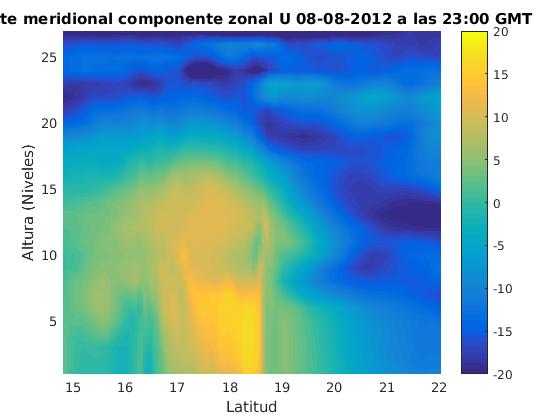
\includegraphics[width=0.35\textwidth]{fig24}
  }\hfill
  \subfloat[ii=29]{%\label{fig:}
  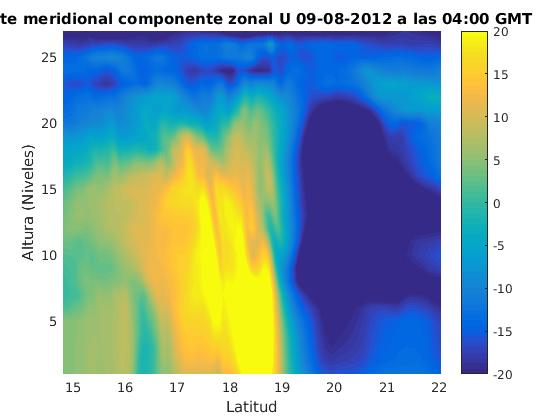
\includegraphics[width=0.35\textwidth]{fig29}
  }\hfill

  \hfill\subfloat[ii=34]{
  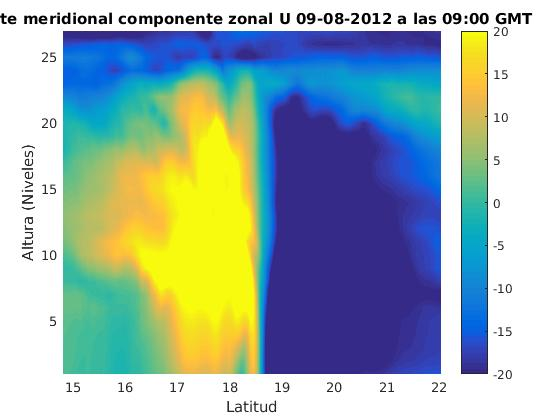
\includegraphics[width=0.35\textwidth]{fig34}
  }\hfill
  \subfloat[ii=39]{%\label{fig:}
  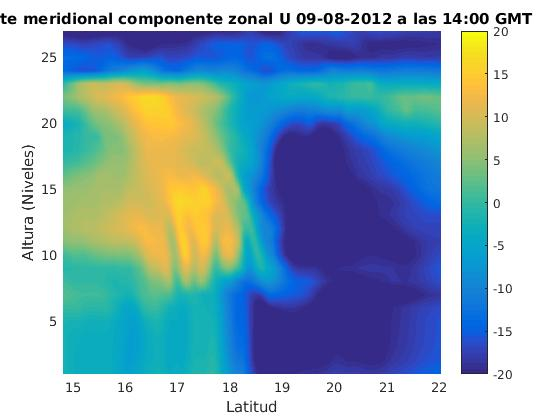
\includegraphics[width=0.35\textwidth]{fig39}
  }\hfill
  \caption{Evoluci\'on de la componente $U$ en un corte meridional (longitud fija $\approx$ 94$^o$)}%
\label{fig:uno}
\end{figure}
%%%%%